\documentclass[a4paper]{article}
\usepackage[utf8]{inputenc}
\usepackage[english]{babel}
\usepackage{amsmath} % per ambienti tipo cases
\usepackage{mathtools}
\usepackage{siunitx}
\usepackage{graphicx} % per includere figure
%\usepackage{subfigure}
\usepackage{booktabs} % per le tabelle
\usepackage{caption}
\usepackage{fancyhdr}
\usepackage{hyperref}
\usepackage[section]{placeins}
\usepackage{microtype}
\usepackage{caption}
\usepackage{subcaption}
\captionsetup[subfigure]{labelfont=rm}
\usepackage{verbatim} %multiline comments
%\usepackage[backend=biber, style=numeric, safeinputenc, sorting=none]{biblatex}
%\addbibresource{source.bib}	% uncomment for bibliography



%opening
\title{}
\author{}

\pagestyle{fancy}
\lhead{Musical Acoustics}
\chead{HL1}
\rhead{10743504, 10751919}
\newcommand{\Rarrow}{\mbox{\Large$\Rightarrow$}}

\begin{document}

\begin{titlepage}	
	\newcommand{\HRule}{\rule{\linewidth}{0.5mm}} % Defines a new command for horizontal lines, change thickness here
	
	\center % Centre everything on the page
	
	%------------------------------------------------
	%	Headings
	%------------------------------------------------
	
	\includegraphics[width=.4\textwidth]{Logo_Politecnico_Milano.png}\\[0.4cm]
	\textsc{\LARGE}\\[0.3cm] % Main heading such as the name of your university/college
	
	\textsc{\large MSc. Music and Acoustic Engineering}\\[1cm] % Minor heading such as course title
	
	\textsc{\Large Musical Acoustics - A.Y. 2020/2021}\\[0.5cm] % Major heading such as course name
	
	%------------------------------------------------
	%	Title
	%------------------------------------------------
	
	\HRule\\[0.4cm]
	
	{\huge\bfseries H4 - Impedance maxima of a compound horn }\\[0.4cm] % Title of your document
	
	\HRule\\[1.5cm]
	
	
	
	{\large\textit{Authors' IDs:}}\\
	10743504, 10751919, % Your name
	%\\ \textsc{Gruppo 11}
	
	%------------------------------------------------
	%	Date
	%------------------------------------------------
	
	\vfill\vfill\vfill % Position the date 3/4 down the remaining page
	
	{\large\today} % Date, change the \today to a set date if you want to be precise
	
	%------------------------------------------------
	%	Logo
	%------------------------------------------------
	
	\vfill\vfill
	%\includegraphics[width=0.2\textwidth]{Politecnico_di_Milano.eps}\\[1cm] % Include a department/university logo - this will require the graphicx package
	
	%----------------------------------------------------------------------------------------
	
	\vfill % Push the date up 1/4 of the remaining page
	
	
\end{titlepage}

\section{Impedance maxima of the pipe}

\begin{figure}[h!]
	\centering
	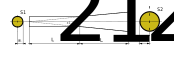
\includegraphics[width=0.8\linewidth]{diagramma.pdf}
	\caption{Scheme of the compound horn system.}
	\label{fig:diag}
\end{figure}

In order to compute the acoustic input impedance of a pipe, one needs to account not only for the air contained in the pipe as an ideal fluid but also for two phenomena occurring around it: the radiation load at the end and the wall losses along its length. The latter is relevant for narrow pipes in particular, but in this case, since the ratio between the pipe's length and the radius of its cross section is $L_1/a_1 = 10$, it is clear that we are not dealing with this condition. Moreover, a common way to characterize the influence of the viscous drag is the ratio of the pipe radius with the boundary layer thickness $r_v$. If this parameter is greater than $10$, it is usually considered safe to neglect the wall losses. Since $r_v \propto \sqrt{f} $, this might not be true at low frequencies; however, in our case, we can see that $r_v$ increases very rapidly from zero and at $\SI{1}{\hertz}$ is already $ \sim 30 $. We assume, therefore, that it is safe for us to ignore such losses in the computation of the impedance. 

Concerning the radiation, instead, we know that its influence on an open-ended pipe is usually not negligible. At low frequency, the strategy that is commonly used to address the study of radiation is to add an end correction $\Delta^{open}$ . At first order in $ka$ the radiation impedance of an open end is equal to the input impedance of an open pipe of length $\Delta^{open}$. We take the value $\Delta^{open} = 0.61 a$; this holds well under the assumption $ka \ll 1 $. However, for us $ka = 1$ at $\sim 1$ kHz, which is well inside the range of frequencies we are interested in.  

\end{document}